\begin{frame}{Experiments}{}
    %  \small{Comparison with using the true I-state, we conducted experiments using 3
    %  environments, and 3 range spaces $\mathcal{R}_{disk}$, $\mathcal{R}_{rect}$,
    %  and  $\mathcal{R}_{drect}$. \\
    %  In each environment we collect the success rate of completing the navigation
    %  task. 
    %  \begin{enumerate}
    %  \item The number of landmarks $N$: between $5$ and $250$ in increments of $5$
    %  \item For each $N$, run the experiment 15 trials with different landmark
    %   distributions by assigning distinct random seeds
    %  \end{enumerate}
    % }
    \only<1>{
    \begin{columns}[T] % align columns
        \begin{column}{.45\textwidth}
            \begin{figure}
                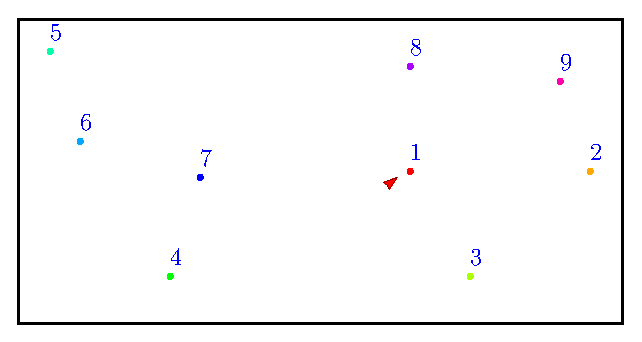
\includegraphics[width=0.9\textwidth]{figs/blank}
            \end{figure}
            \begin{figure}
                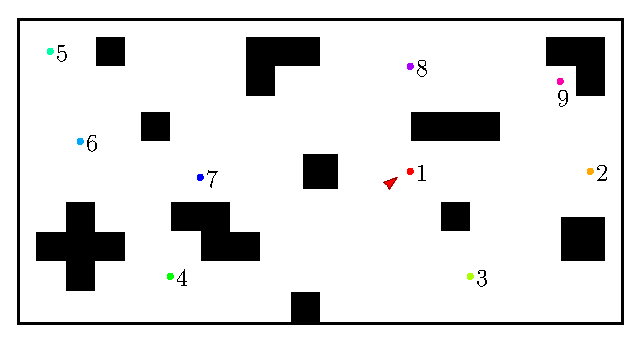
\includegraphics[width=0.9\textwidth]{figs/clutter}
            \end{figure}
        \end{column}%
        \begin{column}{.45\textwidth}
            \begin{figure}
                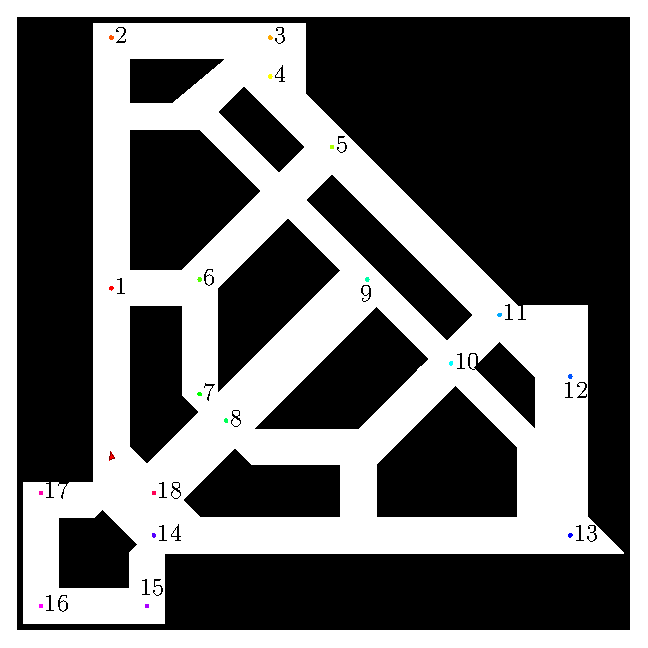
\includegraphics[width=0.9\textwidth]{figs/office}
            \end{figure}
        \end{column}%
    \end{columns}
       
    }
    \only<2>{
        \centering
        \begin{figure}
          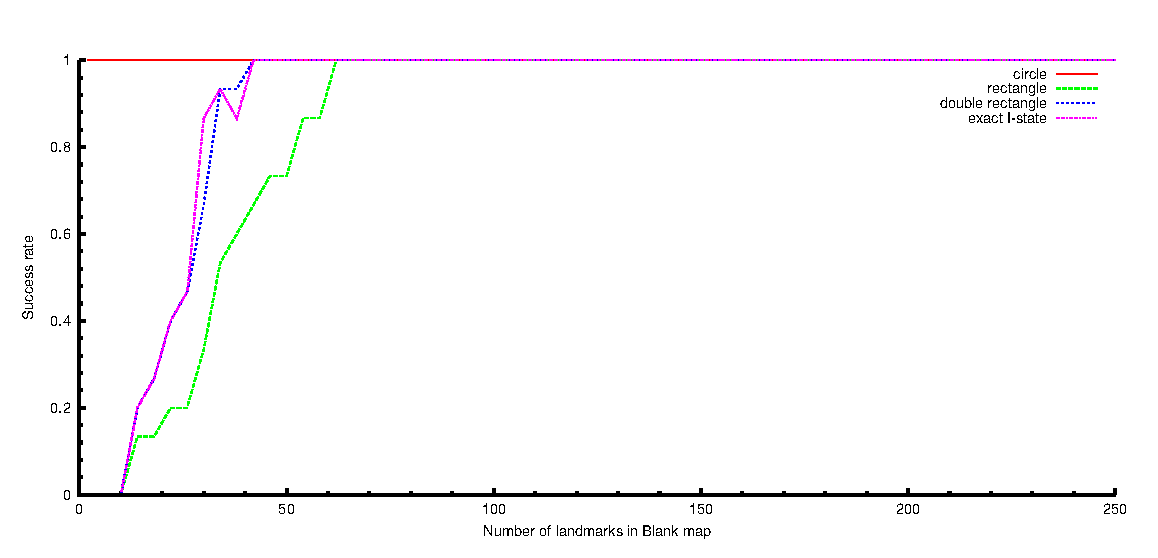
\includegraphics[width=0.9\textwidth]{figs/exp_num_blank_color}%{Data/expnumblank}
        \end{figure}
        \small{Success Rate for the Obstacle-free Environment}
    }
    \only<3>{
        \centering
        \begin{figure}
            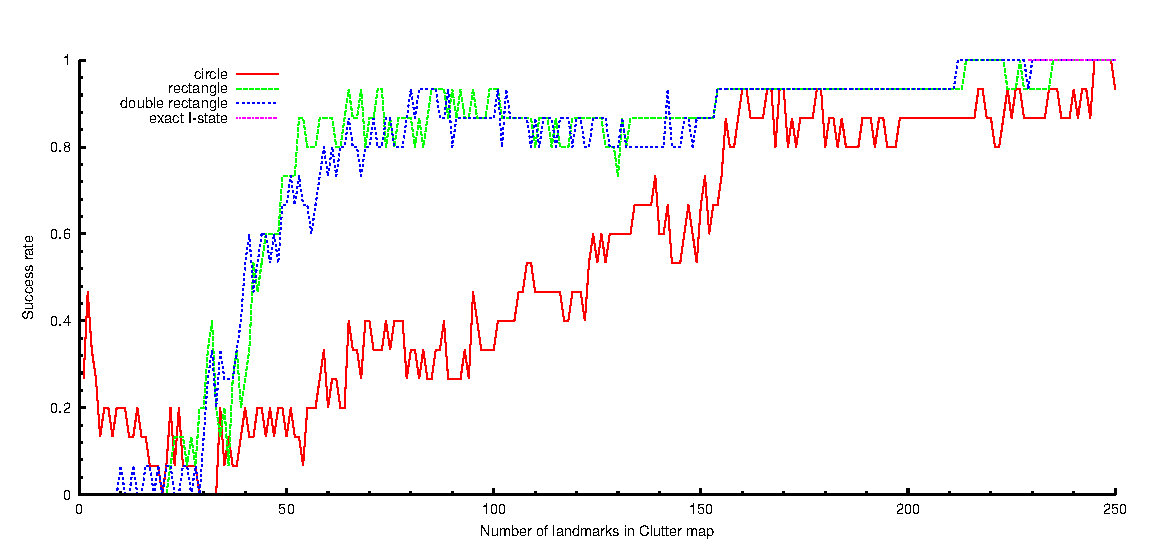
\includegraphics[width=0.9\textwidth]{figs/exp_num_clutter_color}%{Data/expnumclutter}
        \end{figure}
        \small{Success Rate for the Obstacle-cluttered Environment}
    }
    \only<4>{
        \centering
        \begin{figure}
            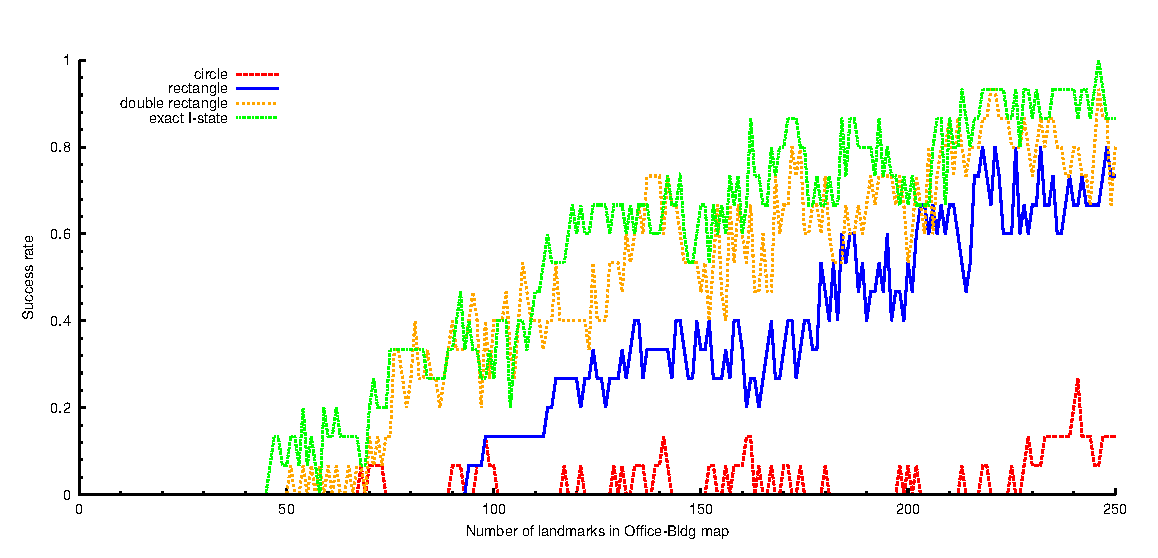
\includegraphics[width=0.9\textwidth]{figs/exp_num_cse_color}%{Data/expnumcse}
        \end{figure}
        \small{Success Rate for the Office-like Environment}
    }
\end{frame}